% !TEX TS-program = pdflatex
% !TEX encoding = UTF-8 Unicode

% This is a simple template for a LaTeX document using the "article" class.
% See "book", "report", "letter" for other types of document.

\documentclass[11pt]{article} % use larger type; default would be 10pt

\usepackage[utf8]{inputenc} % set input encoding (not needed with XeLaTeX)

%%% Examples of Article customizations
% These packages are optional, depending whether you want the features they provide.
% See the LaTeX Companion or other references for full information.

%%% PAGE DIMENSIONS
\usepackage{geometry} % to change the page dimensions
\geometry{a4paper} % or letterpaper (US) or a5paper or....
% \geometry{margin=2in} % for example, change the margins to 2 inches all round
% \geometry{landscape} % set up the page for landscape
%   read geometry.pdf for detailed page layout information

\usepackage{graphicx} % support the \includegraphics command and options

% \usepackage[parfill]{parskip} % Activate to begin paragraphs with an empty line rather than an indent

%%% PACKAGES
\usepackage{booktabs} % for much better looking tables
\usepackage{array} % for better arrays (eg matrices) in maths
%\usepackage{paralist} % very flexible & customisable lists (eg. enumerate/itemize, etc.)
\usepackage{verbatim} % adds environment for commenting out blocks of text & for better verbatim
\usepackage{subfig} % make it possible to include more than one captioned figure/table in a single float
\usepackage{setspace} %paquete para interlineado
\usepackage{graphicx} %para insertar graficos
\usepackage{parskip} % npi de q es
\usepackage{color} %colores


% These packages are all incorporated in the memoir class to one degree or another...

%%% HEADERS & FOOTERS
\usepackage{fancyhdr} % This should be set AFTER setting up the page geometry
\pagestyle{fancy} % options: empty , plain , fancy
\renewcommand{\headrulewidth}{0pt} % customise the layout...
\lhead{}\chead{}\rhead{}
\lfoot{}\cfoot{\thepage}\rfoot{}

%%% SECTION TITLE APPEARANCE
\usepackage{sectsty}
\allsectionsfont{\sffamily\mdseries\upshape} % (See the fntguide.pdf for font help)
% (This matches ConTeXt defaults)

%%% ToC (table of contents) APPEARANCE
\usepackage[nottoc,notlof,notlot]{tocbibind} % Put the bibliography in the ToC
\usepackage{color}
\usepackage[titles,subfigure]{tocloft} % Alter the style of the Table of Contents
\renewcommand{\cftsecfont}{\rmfamily\mdseries\upshape}
\renewcommand{\cftsecpagefont}{\rmfamily\mdseries\upshape} % No bold!

%%% END Article customizations

\usepackage[spanish]{babel}
\usepackage{listings} 
%%% The "real" document content comes below...

\title{Investigación de Lenguajes - HTML}



\author{Fausto Mora\\ Christian Vergara \\ Angel Gonzalez}
\begin{document}
\author{Javier Tibau}

%\date{} % Activate to display a given date or no date (if empty),
         % otherwise the current date is printed 

\maketitle
%\tableofcontents % No hace falta un TOC en un artículo corto

\section{Introducción}
\newcommand{\oops}[1]{\textit{#1}}

\noindent \emph{HTML \oops{{\color{black}Hyper Text Markup Language}}}, es un lenguaje utilizado para crear páginas web, con el se escriben muchas de las estructuras de sitios que existen actualmente en internet.
Los programadores utilizan el lenguaje HTML para crear sus páginas web, estos utilizan programas que generan sitios escritos en este lenguaje y los navegadores que utilizamos a diario muestran las páginas web después de interpretar su contenido HTML.\\

\noindent El lenguaje HTML fue estandarizado por el organismo W3C (\oops{World Wide Web Consortium}) el cual define un estándar para todas las empresas relacionadas con el uso del internet. De esta manera el lenguaje HTML es un lenguaje universalmente reconocido y el cual permite publicar información de manera global.\\

\noindent El eje principal de HTML es la \oops{referenciación} , es decir, para insertar contenido multimedia como fotos, música, videos, archivos, etc , estos no van dentro del código de la página, sino que se hace referencia a los mismos que se encuentran en una ubicación externa. El navegador que interpreta el código HTML une todos estos archivos mostrando así, una página final, mientras que el proceso de creación del código HTML contiene unicamente texto. Ya que éste es un lenguaje estandar es necesario que todos los navegadores ejecuten de la misma manera el código.\\

\noindent A lo largo del desarrollo de HTML, éste ha incorporado diferentes características para adaptarlo a nuevas plataformas (smartphones, tablet, etc), Estos cambios son añadidos a los navegadores cada vez que estos lanzan una nueva versión o actualización. Para la correcta interpretación de una nueva versión de HTML es necesario que los navegadores esten actualizados. Por el contrario las versiones actuales de navegadores por lo general mantienen la interpretación de versiones anteriores de HTML, para poder visualizar el contenido de aplicaciones desarrolladas por las mismas, aunque la apariencia no sea moderna.\\



\section{Características}

\noindent 1.- Lenguaje de facil comprensión.\\
2.- Puede ser creado/modificado en algun editor de textos básico.\\
3.- Es un lenguaje basado en el uso de etiquetas o tags, las cuales determinan el inicio/ cierre de una determinada propiedad en la pagina.\\
4.- La creacion de la pagina se subdivide en dos: cabecera y cuerpo, dentro de instrucciones de inicio/fin.\\ 
5.- Es un lenguaje que permite crear una aplicacion de manera correctamente estructurada.\\
6.- Al ser un lenguaje estandar es interpretador por cualquier navegador en la actualidad.\\
7.- El contenido multimedia que se visualiza en la aplicacion desarrollada en HMTL se encuentra fuera del código, HTML hace referencia a el mismo, y es visualizado cuando el navegador ejecuta el mismo.\\
8.- No es un lenguaje como Java, C++, o C, HTML solo permite crear páginas de formato electronico, aunque en la actualidad existen otros complementos y versiones que incorporan sofisticadas herramientas para la creacion de páginas con una excelente presentación y a su vez una agradable navegación.\\


\section{Historia}

\noindent Fue el físico Tim Berners-Lee (quien laboraba en el CERN, Organización Europea para la Investigación NUclear por sus siglas en ingles) quien dió inicio a la historia del lenguaje HTML a finales de la década de los 80's. Para entonces, ya había nacido el concepto de "hipertexto", el cual era un sistema capaz de dejar que los usuarios accedan a información relacionado con los documentos que estaban consultando, lo que hoy serían los enlaces de las páginas web.\\

\noindent Tras proponer un nuevo sistema de "hipertexto", Tim Berners-Lee empezó el desarrollo de HTML a partir de SGML (\oops{Standar Generalized Markup Language}), que era un estándar ISO de 1986 empleado para la organización y etiquetado de textos, es decir que servía para especificar las reglas de etiquetado de documentos. HTML toma un conjunto de etiquetas existentes en SGML, sin embargo incluye las implementadas por su creador. Luego de finalizar su desarrollo, Tim Berners-Lee lo dió a conocer en  una convocatoria que tenía como fin recibir propuestas referentes al desarrollo de un sistema de "hipertexto" para Internet.\\

\noindent Entre los años 1990 y 1993 aparecen las primeras versiones de HTML, las cuales no estaban estandarizadas debido a que su uso no estaba muy extendido. Fue en 1991 cuando se publicó el primer documento con la descripción del lenguaje HTML nombrado HTMLTags (\oops{Etiquetas HTML}). EL primer intento de estandarización se da cuando nace HTML 1.0 y esta presente en un documento escrito por Tim Berners-Lee y Daniel Conolly. Esta primera versión de HTML no disponía de elementos indispensables para las páginas web actuales tales como tablas y formularios.\\

\noindent En 1993 se empezó a trabajar en la especificación de la siguiente versión de HTML, llamado HTMLplus (HTML+) pero que nunca llego a estandarizarse. La principal novedad de esta versión de HTML radica en la presencia de tablas y formularios, por primera vez en la historia del Lenguaje. Aunque en esta versión del lenguaje se intentó agregar la característica de incluir fórmulas matemáticas, esta nunca se dió. En cambio dió lugar al origen de un nuevo lenguaje llamado MathML. El único navegador capaz de aceptar etiquetas de HTML+ fue el llamado Arena, que fue creado con el fin de probar sus características.\\

\noindent En 1994 es fundado el W3C, que se encarga hasta hoy del desarrollo de las tecnologías que se usan en la web. Ya en 1995 nace HTML 2.0, el primero de todos es ser estandarizado. A pesar de ello, este proyecto no era ampliamente recomendado por el W3C, ya que era un proyecto \oops{Request-for-Coments}. En estos tiempos se dió a conocer la llamada guerra de los navegadores entre Microsoft y Netscape.\\

\noindent EN 1997 se publica HTML 3.2 conocida como la primera versión estandarizada de HTML por la W3C y a finales de 1999 se publicaba la última versión de HTML de ese entonces, HTML 4.1.\\

\noindent A partir de entonces el W3C decidió abandonar el desarrollo de HTML concentrando su gestión en el desarrollo de XML, que es considerado un meta lenguaje, ya que su objetivo es definir reglas para la implementación de otros lenguajes, es decir, que era una versión mejorada de SGML.\\

\noindent En Enero del 2000 se dió a conocer XHTML, que no era mas que una reimplementación de HTML 4 utilizando los estándares fijados en XML 1.0. Este último era practicamente igual a HTML 4.01, sin embargo daba reglas más estrictas para que un documento sea considerado válido. Por ser un lenguaje muy estricto XHTML no triunfó.\\

\noindent Para el año 2004 se formó una organización que se encargaría del desarrollo de un HTML más amigable con la gente. La organización llamada WHATWG estaba formada por Apple, Mozilla y Opera. En este punto la W3C rectifica y se une a WHATWG en su proyecto. Producto de esto se crea HTML 5. Aunque aún es un lenguaje en desarrollo ya existen múltiples desarrolladores que lo usan debido a las novedades que presenta.\\
\section{Tutorial de Instalación}
No podemos olvidar que HTML es un lenguaje y no un programa, y mediante etiquetas de referencia comunica al navegador como interpretar su contenido.  Es decir que HTML lo podemos escribir en cualquier editor de texto ASCII como en el Bloc de Notas de Windows y un navegador web cualquiera para poder visualizarlo. \singlespace

\thinspace Existen programas que ayudan al desarrollo HTML como el  HTMLED o HTML Assistant y tambien encontramos programas que permitern la creacion de paginas web soportando el lenguaje HTML sin la necesidad de escribir una linea de codigo como el Adobe Dreamweaver y MAGIX Web Designer. 

\section{Ejemplos del Codigo:}


\begin{center}
En la imagen (\ref{fig:5.1})  podemos observar un sencillo codigo html 
\end{center}


\begin{figure}[htb]
\centering
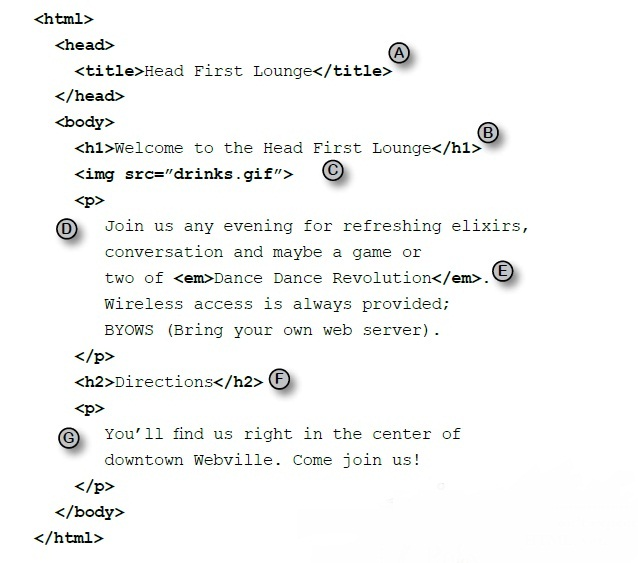
\includegraphics[width=0.7\textwidth]{imagenes/img1.png}
\caption{Codigo HTML}
\label{fig:5.1}
\footnote{Head First HTML book}
\end{figure}

\singlespace

\begin{center}
En la imagen (\ref{fig:5.2}) tambien observar la generacion del codigo al ser traducido por un navegador
\end{center}

\begin{figure}[htb]
\centering
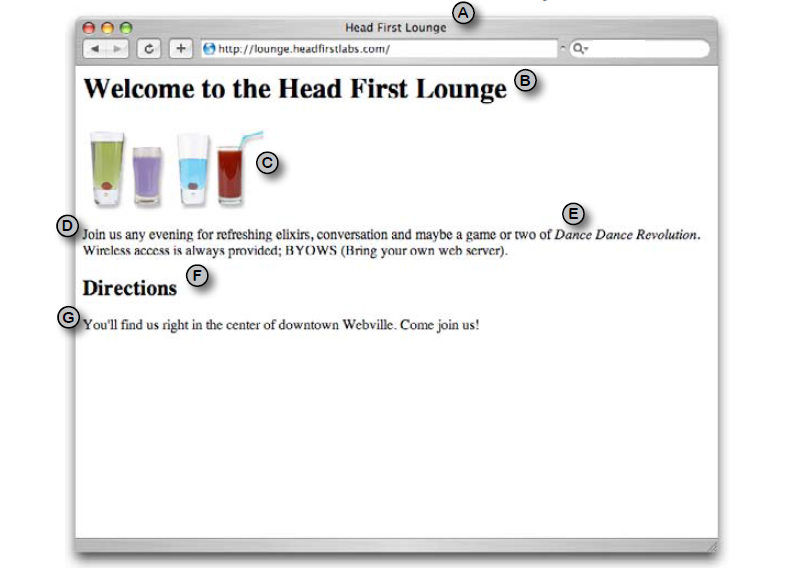
\includegraphics[width=0.7\textwidth]{imagenes/img2.png}
\caption{Codigo HTML ejecutado por navegador}
\label{fig:5.2}
\footnote{Head First HTML book}
\end{figure}


\section{Hola Mundo Ejemplo:}

\begin{center}
En la imagen (\ref{fig:6.1}) observamos el ejemplo Hola Mundo y en la imagen  (\ref{fig:6.2}) podemos visualizar el codigo que genero aquella presentacion
\end{center}


\begin{figure}[htb]
\centering
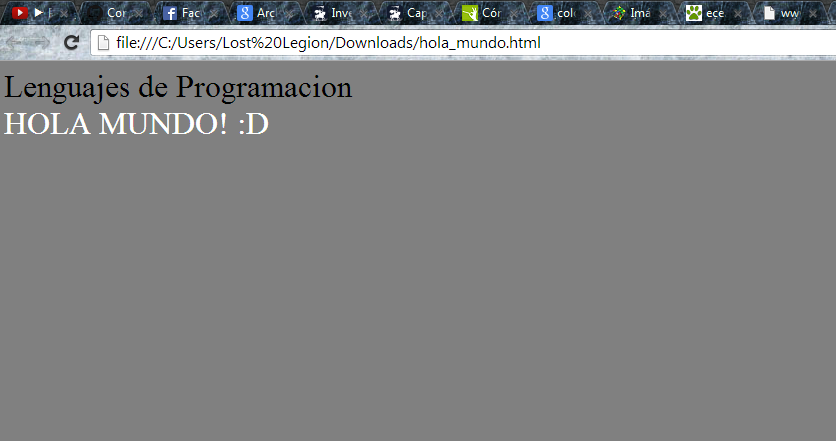
\includegraphics[width=0.8\textwidth]{imagenes/Hola_Mundo.png}
\caption{Hola Mundo ejemplo}
\label{fig:6.1}
\end{figure}


\begin{center}

\end{center}

\begin{figure}[htb]
\centering
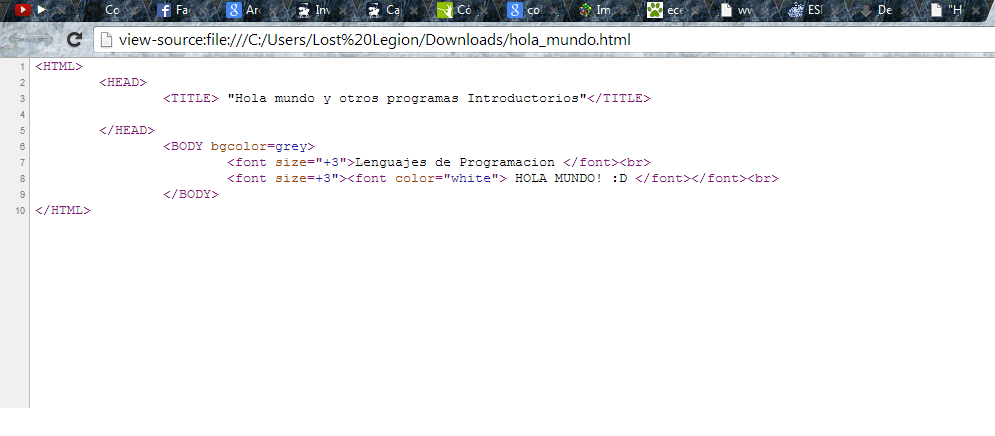
\includegraphics[width=0.8\textwidth]{imagenes/Hola_MundoCod.png}
\caption{Codigo HTML del "Hola Mundo"}
\label{fig:6.2}
\end{figure}





\end{document}
